\section{Optimizing applications}

\begin{frame}
\frametitle{Measuring: strace}
\begin{itemize}
	\item Allows to trace all the system calls made by an
              application and its children.
	\item Useful to:
	\begin{itemize}
		\item Understand how time is spent in user space
		\item For example, easy to find file open attempts (\code{open()}),
		      file access (\code{read()}, \code{write()}), and
		      memory allocations (\code{mmap2()}). Can be done
		      without any access to source code!
		\item Find the biggest time consumers
		      (low hanging fruit)
		\item Find unnecessary work done in applications
		      and scripts. Example: opening the same file(s)
		      multiple times, or trying to open files that
		      do not exist.
	\end{itemize}
	\item Limitation: you can't trace the \code{init} process!
\end{itemize}
\end{frame}

\begin{frame}[fragile]
  \frametitle{strace}
  \begin{columns}
  \column{0.75\textwidth}
  \small
  System call tracer - \url{https://strace.io}
  \begin{itemize}
  \item Available on all GNU/Linux systems\\
        Can be built by your cross-compiling toolchain generator or by your build system.
  \item Allows to see what any of your processes is doing: accessing files, allocating memory...
        Often sufficient to find simple bugs.
  \item Usage:\\
    \code{strace <command>} (starting a new process)\\
    \code{strace -p <pid>} (tracing an existing process)\\
    \code{strace -c <command>} (statistics of system calls taking most time)
  \end{itemize}
  See \href{https://man7.org/linux/man-pages/man1/strace.1.html}{the strace manual} for details.
  \column{0.25\textwidth}
  \includegraphics[height=0.7\textheight]{common/strace-mascot.png}\\
  \tiny Image credits: \url{https://strace.io/}
  \end{columns}
\end{frame}

\begin{frame}[fragile]
  \frametitle{strace example output}
  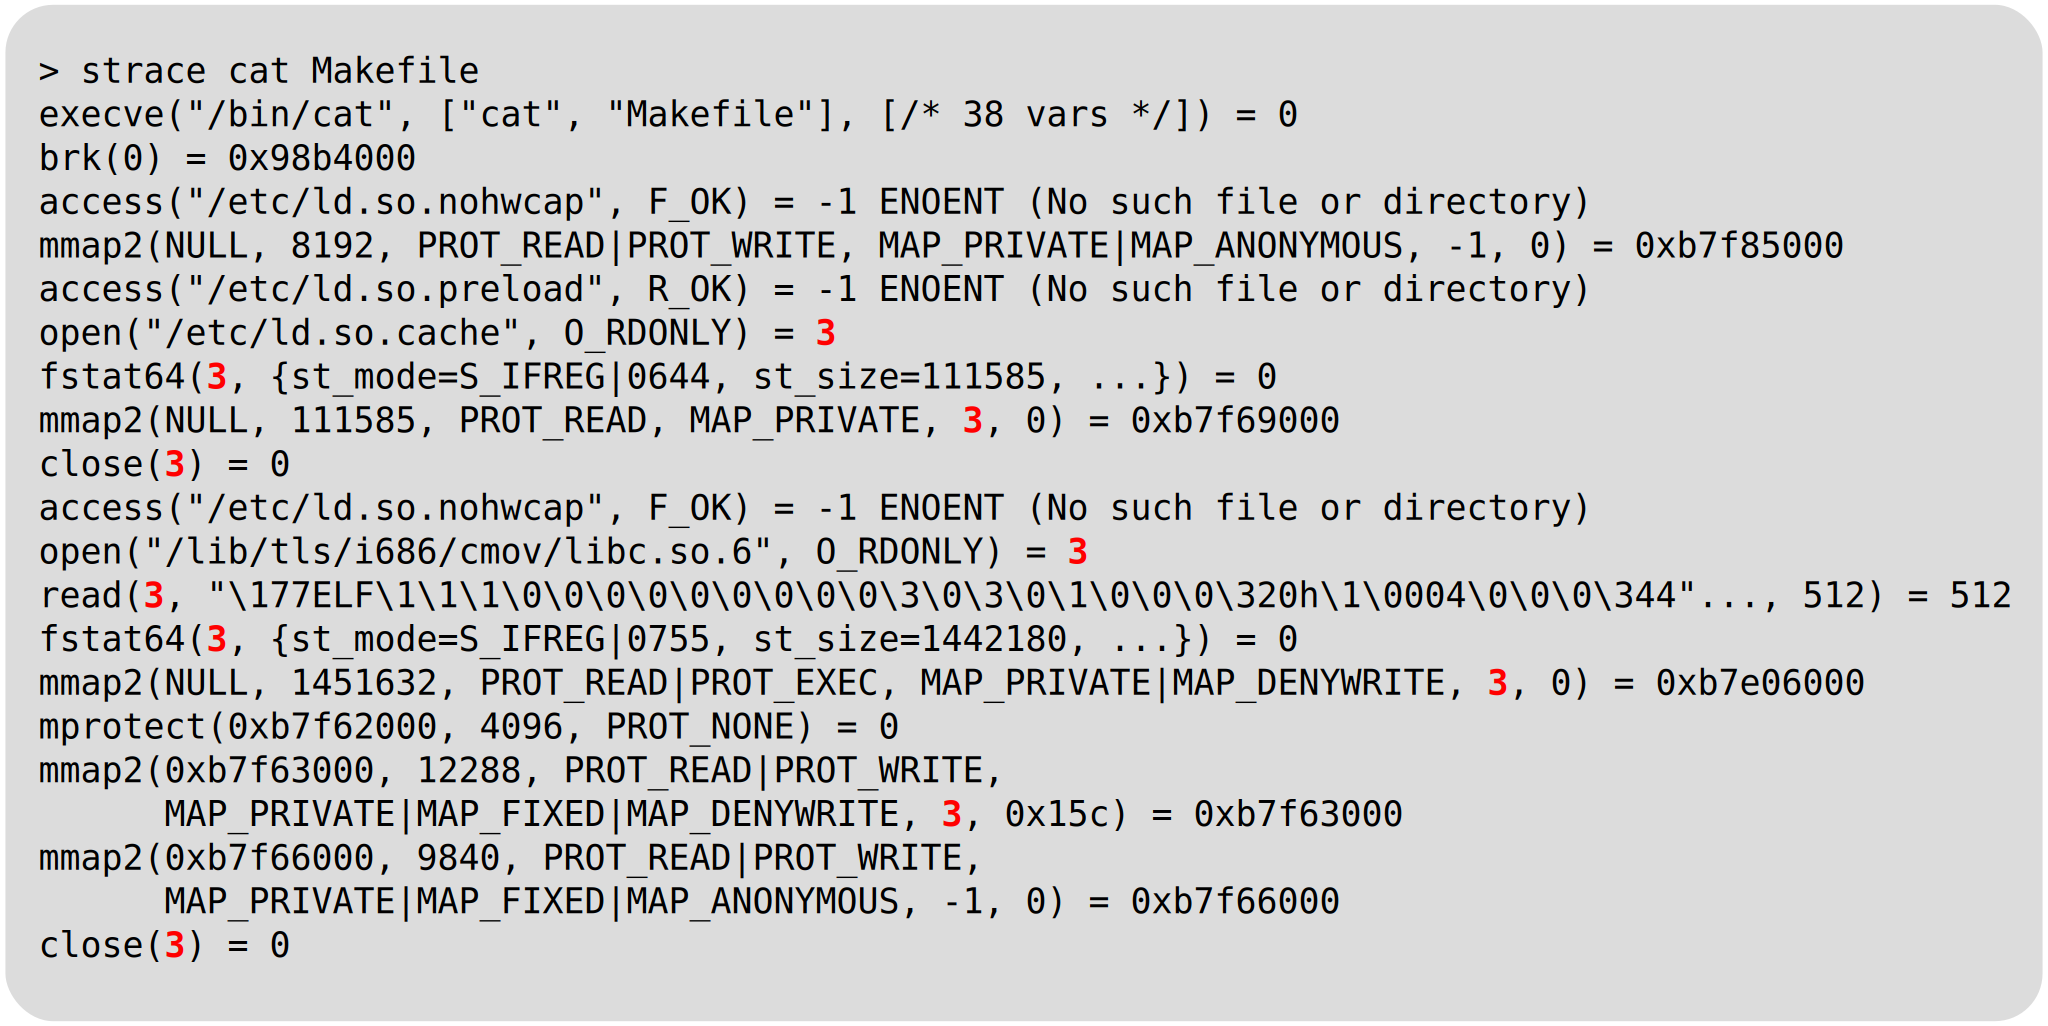
\includegraphics[height=0.75\textheight]{common/strace-output.pdf}\\
  Hint: follow the open file descriptors returned by \code{open()}.
  This tells you what files are handled by further system calls.
\end{frame}

\begin{frame}[fragile]
  \frametitle{strace -c example output}
  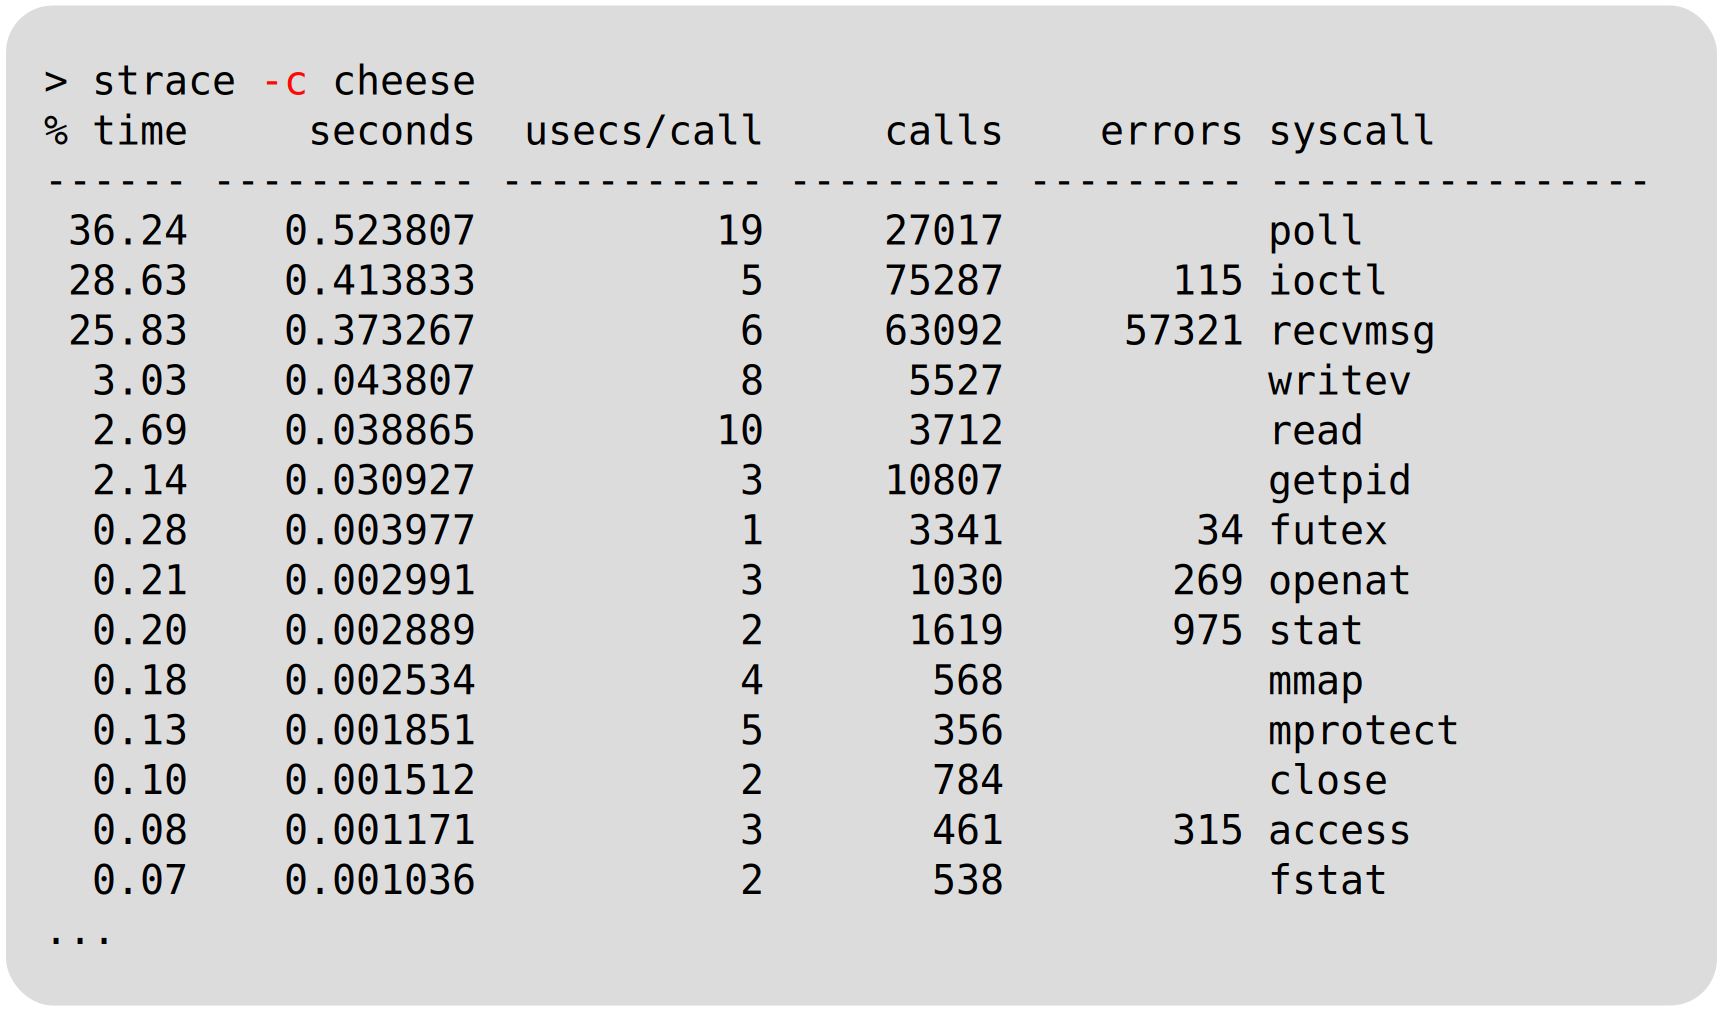
\includegraphics[height=0.8\textheight]{common/strace-c-output.pdf}
\end{frame}


\begin{frame}
\frametitle{oprofile}
A system-wide profiler
\begin{itemize}
	\item Two ways of working: {\em legacy} mode and {\em
              perf\_events} mode
	\item {\em legacy} mode:
	\begin{itemize}
		\item Low accuracy, use a kernel driver to profile
		\item \kconfig{CONFIG_OPROFILE}
		\item User space tools: \code{opcontrol} and \code{oprofiled}
	\end{itemize}
	\item {\em perf\_events} mode:
	\begin{itemize}
		\item Uses hardware performance counters
		\item \kconfig{CONFIG_PERF_EVENTS} and \kconfig{CONFIG_HW_PERF_EVENTS}
		\item User space tools: \code{operf}
	\end{itemize}
\end{itemize}
\end{frame}

\begin{frame}[fragile]
\frametitle{oprofile: usage}
\begin{itemize}
	\item {\em legacy} mode:
	\begin{block}{}
\begin{verbatim}
opcontrol --vmlinux=/path/to/vmlinux # optional step
opcontrol --start
/my/command
opcontrol --stop
\end{verbatim}
	\end{block}
	\item {\em perf\_events} mode:
	\begin{block}{}
\begin{verbatim}
operf --vmlinux=/path/to/vmlinux /my/command
\end{verbatim}
	\end{block}
	\item Get the results with:
	\begin{block}{}
\begin{verbatim}
opreport
\end{verbatim}
	\end{block}
\end{itemize}
\end{frame}

\begin{frame}[fragile]
\frametitle{oprofile}
\begin{block}{}
\tiny
\begin{verbatim}
# opreport
Using /var/lib/oprofile/samples/ for samples directory.
CPU: CPU with timer interrupt, speed 393 MHz (estimated)
Profiling through timer interrupt
          TIMER:0|
  samples|      %|
------------------
     1540 78.3715 no-vmlinux
      105  5.3435 libQtGui.so.4.8.4
       66  3.3588 libc-2.15.so
       64  3.2570 libQtCore.so.4.8.4
       58  2.9517 ld-2.15.so
       45  2.2901 libgobject-2.0.so.0.3000.3
       37  1.8830 libgstreamer-0.10.so.0.30.0
       13  0.6616 libglib-2.0.so.0.3000.3
        9  0.4580 libQtScript.so.4.8.4
        6  0.3053 libgcc_s.so.1
        4  0.2036 libQtDeclarative.so.4.8.4
        4  0.2036 libstdc++.so.6.0.17
        3  0.1527 libpthread-2.15.so
        2  0.1018 busybox
        2  0.1018 libQtSvg.so.4.8.4
        2  0.1018 libQtWebKit.so.4.9.3
        2  0.1018 libgthread-2.0.so.0.3000.3
        1  0.0509 HomeAutomation
        1  0.0509 libQtNetwork.so.4.8.4
        1  0.0509 libphonon_gstreamer.so
\end{verbatim}
\end{block}
\end{frame}

\begin{frame}[fragile]
\frametitle{perf}
\begin{itemize}
	\item Uses hardware performance counters
	\item \kconfig{CONFIG_PERF_EVENTS} and \kconfig{CONFIG_HW_PERF_EVENTS}
	\item User space tool: \code{perf}. It is part of the kernel
		sources so it is always in sync with your kernel.
	\item Usage:
	\begin{block}{}
\begin{verbatim}
perf record /my/command
\end{verbatim}
	\end{block}
	\item Get the results with:
	\begin{block}{}
\begin{verbatim}
perf report
\end{verbatim}
	\end{block}
\end{itemize}
\end{frame}

\begin{frame}[fragile]
\frametitle{perf}
\begin{block}{}
\tiny
\begin{verbatim}
    20.91%  gst-launch-0.10  libavcodec.so.53.35.0        [.] 0x00000000003bdaa1
    15.45%  gst-launch-0.10  libgstflump3dec.so           [.] 0x0000000000014b42
     3.16%  gst-launch-0.10  libglib-2.0.so.0.3600.2      [.] 0x00000000000882c9
     2.99%  gst-launch-0.10  libc-2.17.so                 [.] __memcpy_ssse3_back
     2.37%  gst-launch-0.10  liboil-0.3.so.0.3.0          [.] 0x000000000004417e
     2.24%  gst-launch-0.10  libgobject-2.0.so.0.3600.2   [.] g_type_value_table_peek
     1.53%  gst-launch-0.10  libc-2.17.so                 [.] vfprintf
     1.37%  gst-launch-0.10  libgstreamer-0.10.so.0.30.0  [.] 0x0000000000026fd8
     1.29%  gst-launch-0.10  ld-2.17.so                   [.] do_lookup_x
     0.99%  gst-launch-0.10  libpthread-2.17.so           [.] pthread_mutex_lock
     0.98%  gst-launch-0.10  libgobject-2.0.so.0.3600.2   [.] g_type_check_value
     0.93%  gst-launch-0.10  libgstavi.so                 [.] 0x00000000000119f9
     0.88%  gst-launch-0.10  libgstreamer-0.10.so.0.30.0  [.] gst_value_list_get_type
     0.85%  gst-launch-0.10  libc-2.17.so                 [.] __random
     0.66%  gst-launch-0.10  [kernel.kallsyms]            [k] clear_page_c_e
     0.62%  gst-launch-0.10  [kernel.kallsyms]            [k] try_to_wake_up
     0.61%  gst-launch-0.10  [kernel.kallsyms]            [k] page_fault
     0.58%  gst-launch-0.10  libgobject-2.0.so.0.3600.2   [.] g_type_is_a
     0.57%  gst-launch-0.10  libc-2.17.so                 [.] __strcmp_sse42
     0.57%  gst-launch-0.10  [kernel.kallsyms]            [k] radix_tree_lookup_element
     0.57%  gst-launch-0.10  libc-2.17.so                 [.] malloc
     0.57%  gst-launch-0.10  libc-2.17.so                 [.] _int_malloc
     0.55%  gst-launch-0.10  libgobject-2.0.so.0.3600.2   [.] g_type_check_instance_is_a
     0.53%  gst-launch-0.10  [kernel.kallsyms]            [k] __ticket_spin_lock
     0.53%  gst-launch-0.10  libgobject-2.0.so.0.3600.2   [.] g_type_check_value_holds
     0.53%  gst-launch-0.10  libgstffmpeg.so              [.] 0x000000000001e40c
     0.51%  gst-launch-0.10  libgstreamer-0.10.so.0.30.0  [.] gst_structure_id_get_value
     0.50%  gst-launch-0.10  libc-2.17.so                 [.] _IO_default_xsputn
     0.50%  gst-launch-0.10  [kernel.kallsyms]            [k] tg_load_down
\end{verbatim}
\end{block}
\end{frame}

\begin{frame}
\frametitle{Linker optimizations (1)}
Group application code used at startup
\begin{itemize}
        \item Find the functions called during startup, for example using
              the \code{-finstrument-functions} gcc option.
        \item Create a custom linker script to reorder these functions in
              the call order. You can achieve that by putting each function
              in their own section using the \code{-ffunction-sections} gcc
              option.
        \item Particularly useful for flash storage with rather big MTD
              read blocks. As the whole read blocks are read, you end up
              reading unnecessary data.
\end{itemize}
Details:
{\scriptsize
\url{http://blogs.linux.ie/caolan/2007/04/24/controlling-symbol-ordering/}}
\end{frame}

\begin{frame}
\frametitle{Linker optimizations (2)}
\begin{itemize}
\item Here's a very simple way to find the maximum savings you can expect
      from this technique:
      \begin{itemize}
      \item Start the application once and measure its startup time.
      \item Start the application and measure its startup time again.
            Its code should still be in the Linux file cache,
            and the code loading time will be zero.
      \end{itemize}
\item You now know how much time it took to load the application code
      (and its libraries) the first time. Linker optimizations will
      save less than this upper limit.
\item You can then decide whether this could be worth the effort.
      Such optimizations are costly, as the way you compile your
      applications has to be modified.
\end{itemize}
\end{frame}


\begin{frame}
\frametitle{Prelink}
\begin{itemize}
\item Prelinking reduces the time needed to start an executable,
      pre-computing the load addresses and link tables generated
      by the dynamic linker, instead of doing this at run time.
\item Be careful of security implications, as executable code is
      always loaded at the same address.
\item Code and paper at
      \url{http://people.redhat.com/jakub/prelink/}
\item No release since 2013 and not supported in Buildroot
      either. However, the Yocto Project maintains a variant supporting
      cross-environments, called {\em prelink-cross}:
      \url{http://git.yoctoproject.org/cgit.cgi/prelink-cross}
\end{itemize}
\end{frame}

\setuplabframe
{Optimizing the application}
{
\begin{itemize}
\item Compile the video player with just the features needed at run
      time.
\item Trace and profile the video player with \code{strace}
\item Observe size savings
\end{itemize}
}

